\documentclass[a4paper, 12pt]{article}
\usepackage[T1]{fontenc}
\usepackage[scale=1,angle=0,opacity=1,color=black!60]{background}
\usepackage{tikzpagenodes}
\usepackage{lastpage}
\usepackage{lmodern}
\usepackage{float}
\usepackage{adjustbox}
\usepackage{amsmath}
\usepackage{nccmath}
\usepackage{url}
\usepackage{listings}
\usepackage{alltt}
\usepackage[section]{placeins}
\usepackage{tocloft}
\usepackage{hyperref}
\usepackage[textwidth=420pt,textheight=630pt]{geometry}
\usepackage[spanish, activeacute]{babel} %Definir idioma español
\usepackage[utf8]{inputenc} %Codificacion utf-8
\usepackage{listings}
\hypersetup{
    colorlinks,
    citecolor=black,
    filecolor=black,
    linkcolor=black,
    urlcolor=blue
}
\renewcommand{\cftsecleader}{\cftdotfill{\cftdotsep}}  % lineas punteadas en la tabla de contenidos
\setlength{\oddsidemargin}{15.5pt}
\backgroundsetup{contents={}} %Saca el 'draft'
\definecolor{mygray}{rgb}{0.95,0.95,0.95}
\lstset{
    basicstyle=\footnotesize,
    backgroundcolor=\color{mygray},         
    breaklines=true,
    breakatwhitespace=true,   
    postbreak=\mbox{\textcolor{red}{$\hookrightarrow$}\space},              
    captionpos=b,                    
    keepspaces=true,                 
    numbers=left,                    
    numbersep=5pt,                  
    showspaces=false,                
    showstringspaces=false,
    showtabs=false,
    tabsize=4,
    language=C,
    frame=none,
    title=\lstname,
}
\def\labelitemi{$\bullet$}

\usepackage{titlesec}
\usepackage{hyperref}

\titleclass{\subsubsubsection}{straight}[\subsection]

\newcounter{subsubsubsection}[subsubsection]
\renewcommand\thesubsubsubsection{\thesubsubsection.\arabic{subsubsubsection}}
\renewcommand\theparagraph{\thesubsubsubsection.\arabic{paragraph}} % optional; useful if paragraphs are to be numbered

\titleformat{\subsubsubsection}
  {\normalfont\normalsize\bfseries}{\thesubsubsubsection}{1em}{}
\titlespacing*{\subsubsubsection}
{0pt}{3.25ex plus 1ex minus .2ex}{1.5ex plus .2ex}

\makeatletter
\renewcommand\paragraph{\@startsection{paragraph}{5}{\z@}%
  {3.25ex \@plus1ex \@minus.2ex}%
  {-1em}%
  {\normalfont\normalsize\bfseries}}
\renewcommand\subparagraph{\@startsection{subparagraph}{6}{\parindent}%
  {3.25ex \@plus1ex \@minus .2ex}%
  {-1em}%
  {\normalfont\normalsize\bfseries}}
\def\toclevel@subsubsubsection{4}
\def\toclevel@paragraph{5}
\def\toclevel@paragraph{6}
\def\l@subsubsubsection{\@dottedtocline{4}{7em}{4em}}
\def\l@paragraph{\@dottedtocline{5}{10em}{5em}}
\def\l@subparagraph{\@dottedtocline{6}{14em}{6em}}
\makeatother

\setcounter{secnumdepth}{4}
\setcounter{tocdepth}{4}


\begin{document}		
	% TÍTULO, AUTORES Y FECHA
	\begin{titlepage}
		\vspace*{\fill}
		\begin{center}
			\Large 75.43 Introducción a los sistemas distribuidos \\
			\Huge Entrega Trabajo Práctico 3: Enlace \\
			\bigskip\bigskip\bigskip
			\large\textbf{Integrantes:} \\
			\begin{center}
				\begin{tabular}{||c | c||} 
					\hline
					Alumno & padron \\ [0.5ex] 
					\hline\hline
					Azcona, Gabriela Mariel & 98363 \\
					\hline
					Avigliano, Patricio Andres & 98861 \\
					\hline
					Blanco, Sebastian Ezequiel & 98539 \\
					\hline
				\end{tabular}
			\end{center}
			\textbf{Fecha de Entrega:} 23/10/2018\\
			\textbf{GitHub:} https://github.com/BlancoSebastianEzequiel/Datacenter\\

		\end{center}
		\vspace*{\fill}
	\end{titlepage}
	\pagenumbering{arabic}
	\newpage
			
	% ÍNDICE
	\tableofcontents
	\newpage
	\pagenumbering{arabic}
	\section{Introducción teórica}
		\begin{figure}[ht]
			\begin{adjustbox}{addcode={
				\begin{minipage}{\width}}{
					\caption{%
						Ejemplo de como seria la topologia con un arbol de altura 3.
						}
				\end{minipage}},rotate=360,center}
				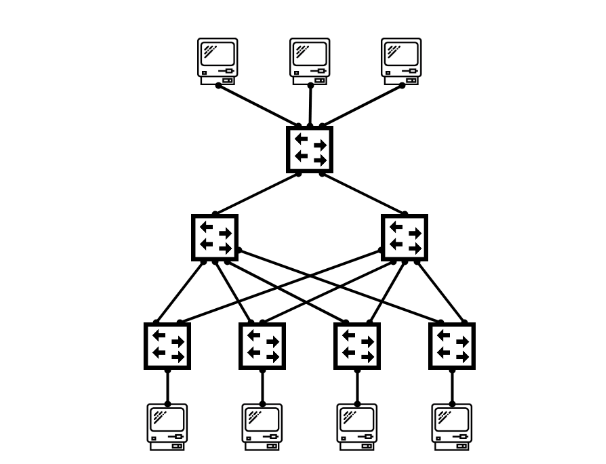
\includegraphics[scale=.6]{pics/topologia-arbol-altura-3.png}
			\end{adjustbox}
		\end{figure}
		\FloatBarrier
	\section{Objetivo}
	\section{Desarrollo}
	\section{Pruebas realizadas}
	\section{Conclusiones}
	\section{Anexos (Código)}
\end{document}
